\scanpage{5}

% l. 1
\mspage{\textcircled{3}}
qu'il est $>2$. Soient \deleted{donc}\inserted{d'abord} $s,t\in E(v)^*$ liés, \inserted{\unsure{ts deux|tous deux}} à $u$ et à $v$.

% ll. 2–3
a) Soient $x\in E(u)^*$, $s\in E(v)^*$, $x$ et $s$ liés. Soit $\unsure{\zeta|z|\xi}\in\deleted{\unsure{E(s)^*}}$ lié à $x$ et $s$. Alors \unsure{$\zeta\in E(w)^*$|$\xi\in E(v)^*$}

% ll. 3–6
\uline{Lemme 5} b) Soient $x,y\in E(u)^*$, $s,t\in E(v)^*$, $x$ et $y$ liés \inserted{(à la fois)} à $s$ et à $t$. [ donc par lemme 3, $x$ et $y$ non liés, $s$ et $t$ non liés). \deleted{\unsure{Soit $\in S$|Soit}} Soient $\zeta,\zeta'$ \deleted{\unsure{$\zeta$ tel}} tels que \deleted{$\unsure{\zeta,(x,s,\zeta)|\xi,(x,s)}$ et $(y,t,$} $\zeta$ lié à $x$ et $s$, $\zeta'$ lié à $y$ et $t$. Alors $\zeta,\zeta'\in E(w)^*$, et $\zeta,\zeta'$ liés.

% ll. 7–11
Démonstration du lemme 5. \deleted{Soit $x$} a) On a $\zeta\in S^*$ car $\zeta\ne u,v,w$ (car $u$ non lié à $s$, $v$ non lié à $x$, $w$ lié ni à $x$ ni à $s$) et $\zeta\notin E(u)^*$, sinon on aurait $\zeta=\sigma(u)$ et $\zeta$ \deleted{\unsure{$\zeta$}} non lié à $s$ par lemme 3, de $=$ $\zeta\notin E(v)^*$, donc $\zeta\in E(w)^*$.

% ll. 12–18
b) Comme $\{x,\unsure{\zeta,s|s,\zeta|\xi,s}\}$ est un triangle, $\zeta'$ est lié à un \deleted{\unsure{pt|et}}\inserted{sommet} et un seul de ce triangle. Or il n'est pas lié à $x$ (sinon $\{\zeta',t\}$ serait arête de deux triangles distincts $\{\zeta',t,x\}$ et $\{\zeta',t,y\}$) ni à $s$ (\deleted{sinon} raison symétrique) donc il est lié à $\zeta'$.

% left beside ll. 13–16
\figure{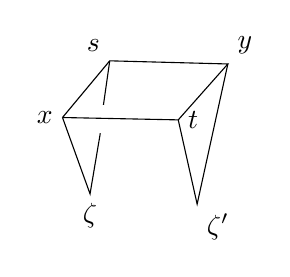
\begin{tikzpicture}[x=1cm,y=1cm]
\draw (0,0) node[left] {$x$} -- (.6,.72) node[above left] {$s$} -- (2.1,.68) node[above right] {$y$} -- (1.47,-.03) node[right] {$t$} -- (0,0);
\draw (0,0) -- (.35,-.97) node[below] {$\zeta$} -- (.48,-.20);
\draw (.52,.16) -- (.6,.72);
\draw (1.47,-.03) -- (1.71,-1.10) node[below right] {$\zeta'$} -- (2.1,.68);
\end{tikzpicture}}

% ll. 19–23
\uline{Dém. du lemme} 4 Supposons $x,y\in E(u)^*$ \inserted{$(x\ne y)$} liés à $s,t,r\in E(v)^*$ distincts. Considérons le triangle $\{x,s,\zeta\}$, donc (lem. 5a) $\zeta\in E(w)^*$, et si $\zeta'=\sigma(t)\in E(w)^*$, en vertu du lemme 5 b) \inserted{appliqué à $(x,y),(s,t)$} $\{\deleted{\unsure{\zeta}}y,t,\zeta'\}$ est un triangle, mais aussi $\{y,r,\zeta'\}$ en regardant $(x,y)\ (s,r)$. Donc

% left beside l. 22
\margin{$x\quad y\qquad s\quad t\quad r$}

% l. 24
$\{y,\zeta'\}$ appartiendrait à 2 triangles, absurde.

% ll. 25–30
\deleted{\uline{Lemme 6}}\inserted{Corollaire 1} Il existe une application \inserted{bijective, \unsure{c.v.c.|c.v., ce|canon.}} et une seule de $\Pi_{22}(P_u)$ dans $\Pi_{22}(P_{\unsure{v|w}})$ ($\Pi_{22}$ indique partitions de type $2,2$) telle que pour \unsure{tte|tout} \deleted{\unsure{partie à 2 élmts de}} \deleted{toute partie à} couple $x,y$ de pts non liés de $E(u)^*$, \deleted{la partition} on ait

% lower left at corollary
\margin{$\pi_u:E_u^*\longrightarrow\underset{\substack{\Vert\\ E_u^*/\mathbb F_2}}{P_u}$}

% bottom
\[
\begin{aligned}
c_{v,u}(\{\pi_u\{x,y\},\complement_{P_u}\pi_u\{x,y\}\}
&=\{\operatorname{supp}\delta_v(x,y),\operatorname{supp}\delta_v(x,y)+\mathbf{1}_{P_v}\}.
\end{aligned}
\]
% archive sheet number: 4
